\documentclass[letterpaper,twoside,12pt]{article}
\usepackage[dvips]{graphicx}
\usepackage[margin=0.8in]{geometry}
\usepackage{caption}
\usepackage{amsmath}
\usepackage{amssymb}
\usepackage[T1]{fontenc}
\usepackage{natbib}
\usepackage{authblk}
%\usepackage{fancyvrb}
%\usepackage{lmodern}
%\usepackage{url}
%\usepackage{times}
\usepackage{textcomp}
\bibliographystyle{agu08}

\newcommand{\ud}{\mathrm d}
\newcommand{\uj}{\mathrm{j}}
\newcommand{\bz}{\mathbf{z}}
\newcommand{\Real}{\mathrm{Re}}
\newcommand{\Imag}{\mathrm{Im}}
\newcommand{\dif}{\mathrm{d}}
\newcommand{\sigsig}{\sigma_1\sigma_2}
\newcommand{\varss}{\varsigma_1\varsigma_2}
\newcommand{\hvarss}{\hat{\varsigma}_1 \hat{\varsigma}_2}
\newcommand{\twodots}{\mathinner {\ldotp \ldotp}}
\newcommand{\midtilde}{\raisebox{0.5ex}{\texttildelow}}

\DeclareMathOperator\erf{erf}

\title{Normality Test for 2-bit Stream Data in Mark-5 Files}

\author[1]{L. V. Benkevitch}
\affil[1]{\small MIT Haystack observatory, Westford, MA 01886, USA.}


\begin{document}

\maketitle

\begin{abstract}
The radio astronomy data from a single dish are recorded in M5B (Mark-5) or VDIF formatted files. The recorded data are supposed to be Gaussian white noise. A corrupted data segment can be spotted at the output of correlation stage. However, the correlation is expensive and vastly increases the bulk of data to be analyzed for spurious parts. Here we consider a problem of finding non~Gaussian (or non-normal) single-dish data segments in M5B files.

The problem may be thought about from a security standpoint. Suppose someone (a malicious character) wishes to hack a system and figures an approach would be to embed some malicious code in. Is it possible to detect the embedded (non-Gaussian) data within a frame or multiple frames before the correlator? Also, even though an algorithm can be determined, is it possible to make its implementation fast enough? The data files are large (up to a hundred gigabytes).

Our solution is based on Pearson's $\chi^2$ test. The null hypothesis states that the data in file  are consistent with the normal distribution. If the data in a part of the file do not pass the test at the significance level 0.05, the null hypothesis is rejected, and the data fragment is flagged.

The algorithm runs on the GPU (Graphics Processing Unit), which provides high speed computations.
\end{abstract}


\section{Quantization and M5B Data Structure}

The analog signal from a single antenna/dish is supposed to be Gaussian noise $N(\mu,\sigma)$ with the expectation $\mu$ and standard deviation (rms) $\sigma$ distributed according to the normal law with the probability density function (PDF):

\begin{equation}
  \label{normal_pdf}
  N(\mu,\sigma) =  \frac{1}{\sigma\sqrt{2\pi}} e^{-\frac{(x-\mu)^2}{2\sigma^2}}.
\end{equation}

The signal is centered to ensure zero $\mu$ and its band is filtered into 16 frequency channels each of which is passed through the 4-level quantizer with the characteristic shown in Fig.~\ref{quant4lvl}.  The quantizer has just three switching thresholds, $-\theta$, 0, and $\theta$, so it is characterized with the only parameter, the adjustable quantization threshold $\pm\theta$. Note that the hardware deals with voltage thresholds, $\pm v_0$, but $\theta$ is expressed in the signal STDs, thus it is dimensionless, $\theta = v_0/\sigma$. The quantizer output only takes four values as in Tab.~\ref{quant_io}. These values are saved in the M5B file.


\begin{figure}[ht!]
  \begin{center}
  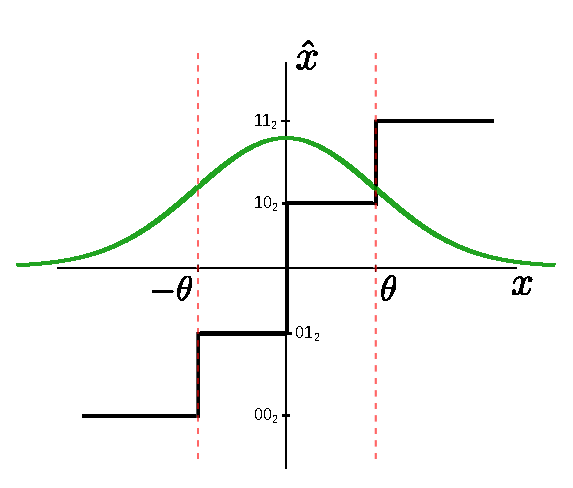
\includegraphics[width=25pc]{fig_4_Level_Quantization_Pattern_impr.eps}
  %\noindent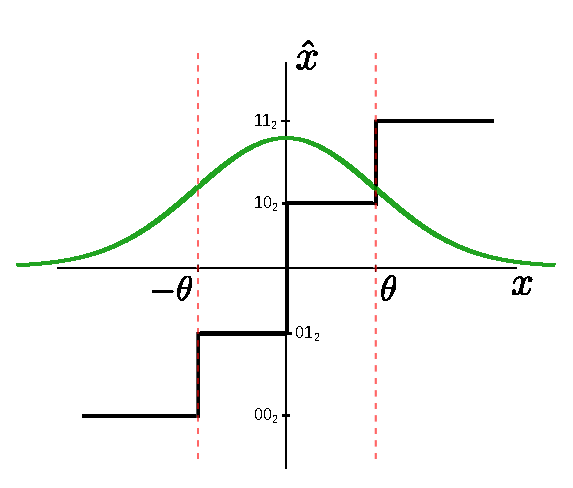
\includegraphics[width=20pc]{fig_4_Level_Quantization_Pattern_impr.eps}
  %\includegraphics[width=\linewidth]{}
  \caption{\small 4-level quantization.}
  \label{quant4lvl}
  \end{center}
\end{figure}


\begin{table}[ht!]
  \begin{center}
    \caption{Quantizer}
    \label{quant_io}
    \begin{tabular}{c|c}
      \textbf{Input, $x$} & \textbf{Output, $\hat{x}$} \\
      \hline
      $-\infty$ to $-\theta$ & 0 \\
      $-\theta$ to 0         & 1 \\
      0 to $\theta$          & 2 \\
      $\theta$ to $+\infty$  & 3 \\
    \end{tabular}
  \end{center}
\end{table}


The M5B file can be considered as an array of 10016-byte frames. Each frame consists of 2504 32-bit words (\verb@unsigned int@ or  \verb@uint@ in C/C++). The first 4 words comprise the frame header, so a frame has 2500 words of pure data. Each 32-bit data word is subdivided into 16 2-bit channels, numbered from 0 to 15. The header contains the sync word \verb@0xdec0de5c@, 23-bit long frame number within second (reset to zero each new second), one flag bit to tag the frame invalid, 8-bit long channel ID, BCD Time Code Word 1 (‘JJJSSSSS’), BCD Time Code Word 2 (‘.SSSS’), and  16-bit CRCC.

Unfortunately, the header does \emph{not} contain the quantization threshold value $\theta = v_0/\sigma$, which is necessary for the statistical testing. In order to estimate $\theta$, the algorithm has to spend precious time on its 1D search as will be described further. 




\section{Statistical Testing Data Normality Using $\chi^2$}

We need to test if the data in each of the 16 channels are sampled from a normally distributed population (the null hypothesis) or not (the alternative hypothesis). In each frame and channel, there are $N=$ 2500 data samples divided into $n=4$ categories by their values, 0, 1, 2, and 3. The counts of data samples in each category form the 4 histogram bins $B_i, i=\overline{0 \twodots 3}$, so $\sum_{i=0}^3 B_i = N$. The Pearson's $\chi^2$ test is based on comparing the observed data counts with the expected (theoretical) counts $E_i, i=\overline{0 \twodots 3}$ obtained from the normal PDF~\eqref{normal_pdf} as $E_i = Np_i$. Here $p_i$ is the probability that a random value sampled from $N(0,\sigma)$ is within the $i$-th interval. The intervals are given in Tab.~\ref{quant_io}, where $i$ is one of the Output values. $\ldots\cdots\ldotp\ldotp$

For each data frame the value of the test-statistic is calculated as

\begin{equation}
  \label{x2_calc}
  X^2 = \sum_{i=0}^3 \frac{(B_i - E_i)^2}{E_i}.
\end{equation}


The $X^2$ test-statistic asymptotically approaches the $\chi^2_{k=3}$ distribution, where $k = n - 1 = 3$ is the number of degrees of freedom. The $\chi^2_{k=3}$ PDF is shown in Fig.~\ref{chi2_pdf}. The statistic $X^2$ is a random value showing how close are the observation frequencies $B_i$ to the perfect, theoretical frequencies $E_i$. The $\chi^2_{k=3}$ PDF has maximum at $X^2=1$ and the mean at $X^2=k=3$. This means that if $X^2$ is distributed as $\chi^2_{k=3}$ its most probable random values will be concentrated somewhere around the mean 3 and not much further. But how much further? The area under the $\chi^2_{k=3}$ PDF curve in Fig.~\ref{chi2_pdf} over an interval $[a,b]$ equals to the probability that the random value will appear within this interval. If we want to be 95\% confident that the data is distributed normally, $X^2$ cannot exceed the critical value $\chi^2_{cr}$ such that the probability for $X^2$ to appear within the interval $[0 \twodots \chi^2_{cr}]$ is $p=0.95$. The critical $\chi^2_{k=3}$ value can be calculated as the value of $\chi^2$ Probability Point Function or PPF, the inverse of the $\chi^2$ Cumulative Distribution Function or CDF. In Python this is done as $\verb@scipy.stats.chi2.ppf(1-alpha, k)@$, where $\alpha = 0.05$ is the level of significance. In our case $\chi^2_{cr} = 7.81$. 

\begin{figure}[ht!]
  \begin{center}
  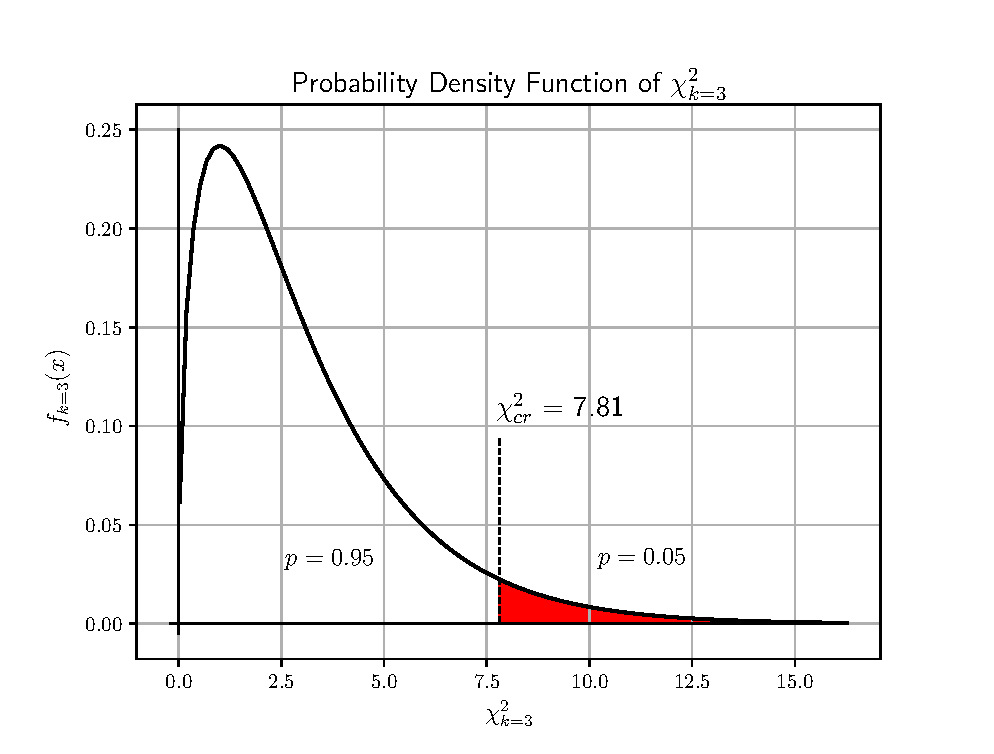
\includegraphics[width=25pc]{fig_chi2_pdf.eps}
  %\noindent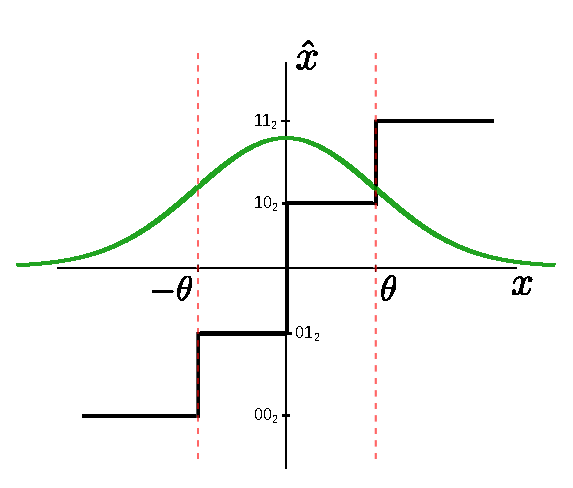
\includegraphics[width=20pc]{fig_4_Level_Quantization_Pattern_impr.eps}
  %\includegraphics[width=\linewidth]{}
  \caption{\small Chi-squared distribution function.}
  \label{chi2_pdf}
  \end{center}
\end{figure}

Thus, our algorithm flags a channel data in frame as non-Gaussian if its $X^2 > 7.81$, the probability of incorrectly rejecting the null hypothesis being $\alpha = 0.05$. In Fig.~\ref{chi2_pdf} this is the red-filled area with the probability 0.05 over the range $[\chi^2_{cr} \twodots +\infty)$. 



\section{Estimation of Quantization Threshold Using 1D Search}

As mentioned, the M5B files do not provide the values of quantization threshold $\theta$, which is continuously being adjusted and can differ from one frame to the next. Assuming the data are sampled from the normally distributed population we can hypothesize that the $\theta_{\text{opt}}$ value that provides the best fit of the observed frequencies $B_i$ to the normal frequencies $E_i$ can be a good estimate of the actual $\theta$ established at the quantization time.

One can notice that the $X^2$ statistics in Eq.~\eqref{x2_calc} is a function of a single variable $\theta$: 

\begin{equation}
  \label{x2_func_of_theta}
  X^2(\theta) = \sum_{i=0}^3 \frac{(B_i - E_i(\theta))^2}{E_i(\theta)},
\end{equation}

where the normal frequencies $E_i$ are dependent on the quantization thresholds positions:

\begin{equation*}
  \label{norm_freq}
  E_{0\twodots3}(\theta) = N \cdot \left[\Phi(-\theta), \; \frac{1}{2}-\Phi(-\theta), \; 
                             \frac{1}{2}-\Phi(-\theta), \; \Phi(-\theta) \right],
\end{equation*}

as shown in Fig.~\ref{npdf_areas}, and $\Phi(x)$ is the normal CDF with $\mu=0$ and $\sigma=1$:

\begin{equation}
  \label{ncdf}
  \Phi(x) = \frac{1}{2} \left[1 + \erf \left( \frac{x}{\sqrt{2}} \right) \right].
\end{equation}


\begin{figure}[ht!]
  \begin{center}
  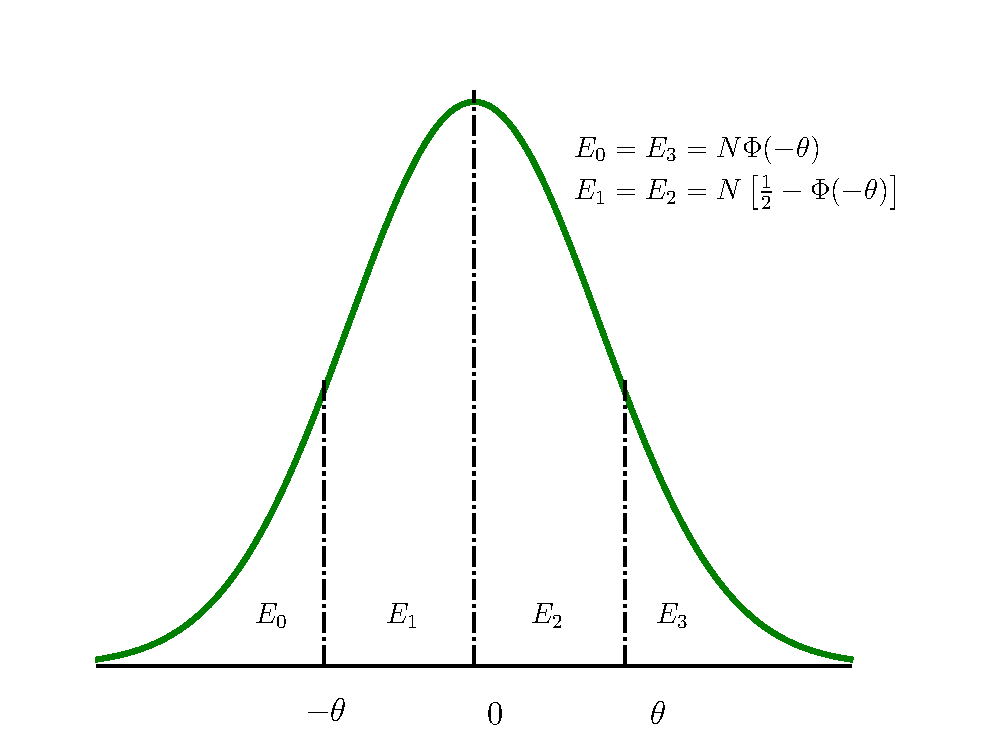
\includegraphics[width=25pc]{fig_npdf_areas.eps}
  \caption{\small  $\theta = 0.7988$, which can be used as an estimate for the actual threshold used in the analog signal quantization.}
  \label{npdf_areas}
  \end{center}
\end{figure}

Fig.~\ref{optimum_theta} shows that the curve $y = X^2(\theta)$ has the only minimum. Thus, the best fit of the normal frequencies $E_i$ to the observed frequencies $B_i$ can be reached at the single $\theta=\theta_\text{opt}$ value that provides minimum to $X^2(\theta)$. 

We have used a fast-converging Brent's algorithm for one-dimensional search. It is a combination of the golden section search at the beginning and the parabolic interpolation when the process is close enough to the minimum.


\begin{figure}[ht!]
  \begin{center}
  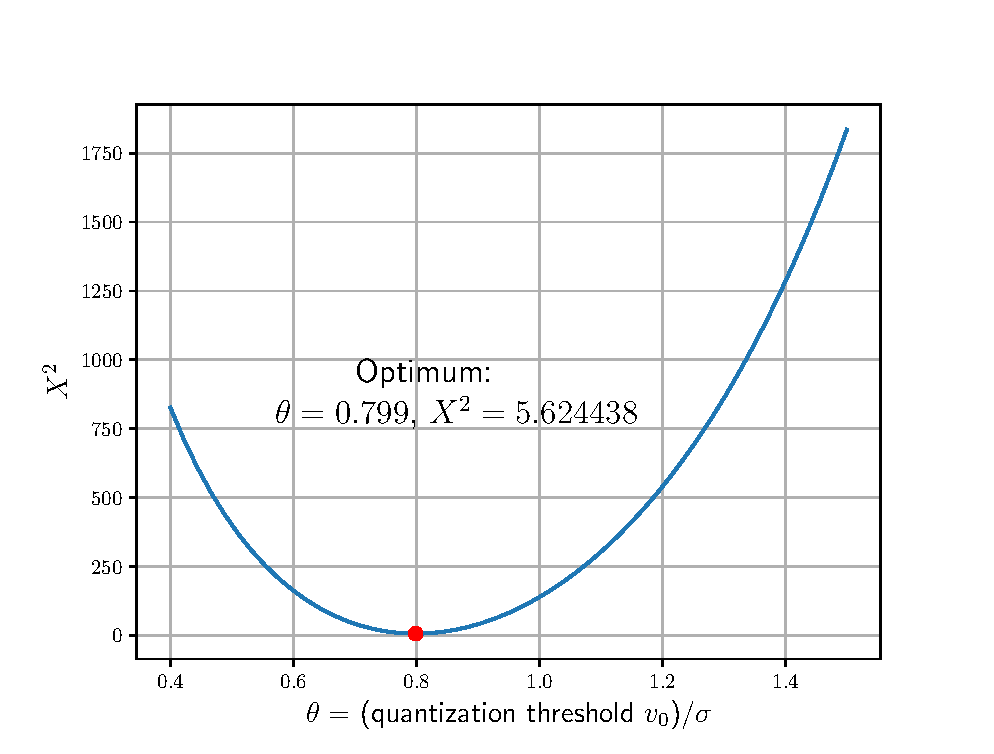
\includegraphics[width=25pc]{fig_optimal_quantization_threshold.eps}
  \caption{\small $X^2(\theta)$ from Eq.~\eqref{x2_func_of_theta} as the measure of error between the observed, $B_i$, and normal, $E_i$ frequencies for the range of quantization tresholds $[0.4 \mathinner{\ldotp\ldotp}1.5]$. The curve has minimum at $\theta = 0.7988$, which can be used as an estimate for the actual threshold used in the analog signal quantization.}
  \label{optimum_theta}
  \end{center}
\end{figure}


\section{Using Graphics Processing Units (GPU)}

The Graphics Processing Units with their hundreds and thousands of processor cores and multiple memory channels allow 1 to 3 orders of magnitude speed-up of the common algorithms. There are two major software frameworks, CUDA and OpenCL. CUDA is developed specifically for the Nvidia GPUs. OpenCL can be used on many parallel architectures. OpenCL is the only option for the AMD GPUs.

In both frameworks, the application code consists of two parts. One part is executed on the host PC. It reads the M5B files, prepares the GPU, uploads there the codes and the M5B data, starts the computations on the GPU, downloads the results from the GPU to the host memory, and saves them to the disk. The other part of code is executed in parallel on the multiple GPU cores. The programs executed on the GPU are called kernels. 

In both frameworks we use single precision floating point arithmetics, which provides the fastest computations.

In the both frameworks, the kernels are written in the C language subsets with some extensions. The host code uses CUDA or OpenCL API. It can be written in C/C++ and some other languages. However, Python is always preferred to make life easier. We use Python wrappers for the both frameworks: PyCUDA and PyOpenCL, and the host part of the NormTest software is written in Python. 

The Python module for normality testing, \verb@gpu_m5b.py@, described in the next section, transfers control to the C kernel previously transferred to the GPU. The kernels are different for different frameworks used. In any individual normality test only two C files are used. Their names start with the following strings: \verb@ker_m5b_gauss_test@ and \verb@fminbndf@. \\

\noindent \verb@ker_m5b_gauss_test*@ defines the test kernel \verb@m5b_gauss_test()@ and the minimized function  \\
\hangindent=0.7cm \verb@calc_chi2()@, which calculates $\chi^2$ between the four bins of standard normal distribution and the four bins with the observation data counts. \\

\noindent \verb@fminbndf*@ implements one-dimensional search for the optimal quantization threshold $\theta_\text{opt}$  \\
\hangindent=0.7cm based on Brent's algorithm. It calls the \verb@calc_chi2()@ function. The search is performed within the bounds $\theta \in [0.5\sigma \twodots 1.5\sigma]$ with the absolute precision \verb@atol@ $=10^{-4}$. Also, the number of iterations is limited to  \verb@maxiter = 20@. \\


In the CUDA framework just the two C files are used: \\

\noindent \verb@ker_m5b_gauss_test.cu@  - test kernel for CUDA; \\
\noindent \verb@fminbndf.cu@ - Brent's algorithm for CUDA. \\

The OpenCL framework requires more options because of the different implementations of OpenCL for different hardware platforms, AMD and Nvidia. Unfortunately, according to OpenCL Specifications, pointers to functions are not allowed, while CUDA does not have this restriction. So, in the OpenCL code for AMD GPU, instead of using this convenient mechanism to pass to the \verb@fminbndf()@ optimizer the pointer to an arbitrary minimized function as its parameter, we have to call \verb@calc_chi2()@ from inside \verb@fminbndf()@. This makes \verb@fminbndf()@ less universal. On the contrary, Nvidia's OpenCL implementation (probably) has an extension allowing this feature. Therefore, there are four OpenCL C files: \\

\noindent \verb@ker_m5b_gauss_test.cl@ - test kernel for Nvidia OpenCL; \\
\noindent \verb@fminbndf.cl@ - Brent's algorithm for Nvidia OpenCL, \\

\noindent and \\

\noindent \verb@ker_m5b_gauss_test_amd.cl@ - test kernel for AMD OpenCL; \\
\noindent \verb@fminbndf_amd.cl@ - Brent's algorithm for AMD OpenCL. \\



\section{Python Module for Normality Testing}

The \verb@gpu_m5b.py@ module defines the only class \verb@Normtest@ that integrates in itself all the normality testing mechanisms. When imported from the \verb@gpu_m5b@ module, \verb@Normtest@ class probes the hardware and automatically determines which framework to use. If it detects an AMD GPU, it uses OpenCL. If an Nvidia GPU is detected, the software uses CUDA. In case both frameworks are installed, it prefers CUDA since it is \midtilde 1.5  times faster than OpenCL. Thus this class provides "transparent" access to the GPU independent of the software framework used. Current version of the software can use only one GPU, however, in future it is possible to employ multiple GPUs on the same motherboard, even using different frameworks. 

The \verb@Normtest@ class provides a "class method" \verb@do_m5b()@ with one argument, a string with M5B filename. It runs the normality test on the available GPU using the software framework selected. If the M5B file is large and it does not fit into either the system RAM or the GPU RAM, it is processed in chunks. The \verb@Normtest@ class is not intended to create multiple class instances (although it is surely possible). Instead, the method \verb@do_m5b()@ is called directly with the class name or its alias. Below is an example procedure of normality tests on several M5B or M5A files: \\

\noindent
\verb@from gpu_m5b import Normtest as nt@  \\
\verb@nt.do_m5b("rd1910_wz_268-1811.m5b")@ \\
\verb@nt.do_m5b("rd1910_ny_269-1413.m5a")@ \\
\verb@nt.do_m5b("rd1910_ny_269-1404.m5a")@ \\
\verb@nt.do_m5b("rd1903_ft_100-0950.m5b")@ \\

The results are saved in 5 binary files. The files have the following names: \\\\
\verb@nt_<data>_<framework>_<m5b_basename>_<timestamp>.bin@, \\\\
\noindent where

\noindent \verb@<data>@ is one of the result types: \\
\indent \verb@bin: dtype=np.float32, shape=(n_frames,16,4)@, 4 histogram bins for 16 channels; \\
\indent \verb@chi2:   dtype=np.float32, shape=(n_frames,16)@, $\chi^2$ for 16 channels; \\
\indent \verb@thresh: dtype=np.float32, shape=(n_frames,16)@, quantization thresholds found
        for 16 channels; \\
\indent \verb@flag:   dtype=np.uint16, shape=(n_frames,16)@, flags for 16 channels; \\
\indent \verb@niter:  dtype=np.uint16, shape=(n_frames,16)@, number of iterations of Brent's
        optimization method used to find the optimal quantization threshold
        for 16 channels;

\noindent \verb@<framework>@ is \verb@cuda@ or \verb@opencl@. \\
\noindent \verb@<m5b_basename>@ is the M5B or M5A file name without extension; \\
\noindent \verb@<timestamp>@ is \verb@YYYYMMDD_HHMMSS@ followed by milliseconds, like \verb@20231015_113649.078@. The timestamp is intended to make the result filename reasonably unique. \\

Empirically, it has been found that the best performance is achieved 
with 8 threads per block (in CUDA terminology), or, which is the same, 
8 work items per work group (in OpenCL terms). However, this number can 
be changed using the \verb@nthreads@ parameter. An example of setting 64 threads per block: \\

\noindent \verb@nt.do_m5b("rd1910_wz_268-1811.m5b", nthreads=64)@ \\


\section{Python Scripts for Analysis of Results}

\subsection{inspect\_nt.py}

This script creates 4x4 plots of 16 histograms for each of the 16 channels. The plots are for one or several (averaged) frames. The histograms are compared with the normal distribution curves showing the vertical borders of the bins at the positions of quantisation threshold estimates, $\pm\theta$. In each subplot both $\theta$ and $\chi^2$ values are printed. The $\chi^2$ values exceeding $\chi^2_{cr} = 7.81$ are printed in red. The data are read from the \verb@*.bin@ files created with the \verb@gpu_m5b_chi2.py@. \\

\noindent Running:

\noindent \verb@%run inspect_nt.py <m5b_filename> <timestamp> <start_frame_#> <#_of_frames> @

The \verb@<timestamp>@ can be any rightmost part of the timestamp before the file extension, \verb@.bin@. The timestamp is present in order to distinguish the \verb@*.bin@ files generated for the same M5B file at different runs. In most cases, providing the last 3 digis (i.e. milliseconds) is enough as long as they refer to the unique group of binary files with normality test results. \\

\noindent Some interesting frames: \\

The histograms are very far from the normal distributions, but most of the $\chi^2$ values
are very small and signal "normality": \\

\noindent \verb@%run inspect_nt.py rd1903_ft_100-0950.m5b 025 97737 1@ \\

These plots are definitely from the uniform distributions, and yet, most
of the $\chi^2$ values are very small and signal "normality". The pearson's
criterion also does not work. \\

\noindent \verb@%run inspect_nt.py rd1903_ft_100-0950.m5b 025 4 1@
\noindent \verb@%run inspect_nt.py rd1903_ft_100-0950.m5b 025 170578 1@
\noindent \verb@%run inspect_nt.py rd1903_ft_100-0950.m5b 025 389930 1@
\noindent \verb@%run inspect_nt.py rd1903_ft_100-0950.m5b 025 6832715 1@ \\

These plots show close to normal histograms with good $\chi^2$ values, i.e.
< 7.81. \\

\noindent \verb@%run inspect_nt.py rd1910_wz_268-1811.m5b 970 200 1@
\noindent \verb@%run inspect_nt.py rd1910_ny_269-1404.m5a 395 7139 1@ \\


%8. plot_25pc_npdf_expectations.py
%
%Plots the normal curve N(0,1) divided vertically into 4 equal areas under the 
%curve (25%-bins). The division lines are at -0.6745, 0, and +0.6745. 
%For each of the areas, the math expectations are computed, they are at 
%    -1.27, -0.32, 0.32, and 1.27 (in STDs). 
%Thse are the most probable analog signal values before the quantization with
%the *ideal* thresholds -0.6745, 0, and +0.6745, which provide the uniform 
%arrangement of the discrete signal in the 4 bins.  
%%
%4. plot_m5b_thrange.py
%
%Plots squared error (the residual) between M5B Data and four bins of the
%standard normal distribution over the range [0.4 .. 1.5] of input sample
%thresholds. The plot obviously has its minimum at the threshold +-0.817/STD
%marked with the red dot.
%
%
%5. test_m5b.py
%
%Calculates the observed $\chi^2$ and compares it with the $\chi^2$ critical value at
%the significance level 0.05 for the degrees of freedom 3 (we have 4 bins,
%so df = 4 - 1 = 3).
%
%Plots histograms of the observed data and the theoretical normal distribution
%to compare.
%
%Running:
%%run test_m5b.py <m5b_filename>
%
%
%6. plot_m5b_hist.py
%
%Plots two histograms of the results from gpu_m5b.py for the whole 
%M5B (or M5A) file: 
%6.1. Distribution of $\chi^2$ and a red marker showing position of the critical
%     $\chi^2$ value (7.81), as well as the percent of $\chi^2$ exceeding it.
%6.2. Distribution of the optimal quantization thresholds and a red marker
%     showing position of the critical threshold value (0.6745 rms), as well as
%     the percent of the thresholds that failed to reach it.
%
%

%
%
%9. skew_kurt.py
%
%Calculates skewness and kurtosis of a frame in M5B or M5A file.
%The data positions (in STDs) are assumed at the 25%-bin math expectations,
%  mu0 = -1.27, mu1 = -0.32, mu2 = 0.32, and mu3 = 1.27.

\begin{thebibliography}{99}

\bibitem[{\textit{Kiefer}(1953)}]{Kiefer1953} 
{Kiefer}, J.~L. (1953), {Sequential minimax search for a maximum}, \textit{Proceedings of the American Mathematical Society}, \textit{4}, (3), 502-–506, DOI:10.1109/TIT.1967.1053965.

%\bibitem[{\textit{{Brown}}(1967)}]{Brown1967}
%{Brown}, J.~L. (1967), {A Generalized Form of Price's Theorem and Its Converse}, \textit{IEEE Transactions on Information Theory}, \textit{13}, 27--30, \doi{10.1109/TIT.1967.1053965}.
%
%\bibitem[{\textit{{Cooper}}(1970)}]{Cooper1970}
%{Cooper}, B.~F.~C. (1970), {Correlators with two-bit quantization},
%  \textit{Australian Journal of Physics}, \textit{23}, 521--527.
%
%\bibitem[{\textit{{Greisen}}(2003)}]{Greisen2003}
%{Greisen}, E.~W. (2003), {AIPS, the VLA, and the VLBA}, \textit{Information
%  Handling in Astronomy - Historical Vistas}, \textit{285}, 109,
%  \doi{10.1007/0-306-48080-8\_7}.
%
%\bibitem[{\textit{{Hagen} and {Farley}}(1973)}]{Hagen1973}
%{Hagen}, J.~B., and D.~T. {Farley} (1973), {Digital-correlation techniques in
%  radio science.}, \textit{Radio Science}, \textit{8}, 775--784,
%  \doi{10.1029/RS008i008p00775}.
%
%\bibitem[{\textit{{Johnson} et~al.}(2013)\textit{{Johnson}, {Chou}, and
%  {Gwinn}}}]{Johnson2013}
%{Johnson}, M.~D., H.~H. {Chou}, and C.~R. {Gwinn} (2013), {Optimal Correlation
%  Estimators for Quantized Signals}, \textit{Astrophysical Journal},
%  \textit{765}, 135, \doi{10.1088/0004-637X/765/2/135}.
%
%\bibitem[{\textit{{Kulkarni} and {Heiles}}(1980)}]{Kulkarni1980}
%{Kulkarni}, S.~R., and C.~{Heiles} (1980), {How to obtain the true correlation
%  from a 3-level digital correlator}, \textit{Astronomical Journal},
%  \textit{85}, 1413--1420, \doi{10.1086/112815}.
%
%
%
%\bibitem[{\textit{Bracewell}(1986)}]{Bracewell1986}
%Bracewell, R.~N. (1986), \textit{{The Fourier Transform and Its Applications}},
%  2nd, revised ed., 474 pp., WCB/McGraw-Hill, Boston, Massachusetts.
%
%\bibitem[{\textit{Bracewell}(1986)}]{Bracewell1986}
%Bracewell, R.~N. (1986), \textit{{The Fourier Transform and Its Applications}},
%  2nd, revised ed., 474 pp., WCB/McGraw-Hill, Boston, Massachusetts.
%


\end{thebibliography}



\end{document}



